% Compile with XeLaTeX, TeXLive 2013 or more recent
\documentclass{beamer}

% Base packages
\usepackage{fontspec}
\usepackage{xunicode}
\usepackage{xltxtra}

\usepackage{amsfonts}
\usepackage{amsmath}
\usepackage{longtable}
\usepackage{csquotes}
\usepackage{standalone}

% Setup fonts
\newfontfamily\russianfont{CMU Serif}
\setromanfont{CMU Serif}
\setsansfont{CMU Sans Serif}
\setmonofont{CMU Typewriter Text}

% Setup Russian hyphenation. NOTE: this declaration *must* come after fontspec's font declarations,
% or a mysterious (but harmless in other respects) error "Improper `at' size (0.0pt), replaced by 10pt." would appear.
\usepackage{polyglossia}
\defaultfontfeatures{Scale=MatchLowercase, Mapping=tex-text}

\setdefaultlanguage[spelling=modern]{russian} % for polyglossia
\setotherlanguage{english} % for polyglossia

% Vector drawings
\usepackage{tikz}
% \usetikzlibrary{shapes, calc, arrows, fit, positioning, decorations, patterns, decorations.pathreplacing, chains, snakes}
\usetikzlibrary{shapes, calc, arrows, decorations.markings, decorations.pathreplacing, decorations.pathmorphing, decorations, patterns, chains, snakes, backgrounds, positioning, fit, shadows}
% \usepackage[siunitx]{circuitikz}

% Be able to insert hyperlinks
\usepackage{hyperref}
\hypersetup{colorlinks=true, linkcolor=black, filecolor=black, citecolor=black, urlcolor=blue , pdfauthor=Grigory Rechistov <grigory.rechistov@phystech.edu>, pdftitle=Курс «Программное моделирование вычислительных систем»}
% \usepackage{url}

% Misc optional packages
\usepackage{underscore}
\usepackage{amsthm}

% A new command to mark not done places
\newcommand{\todo}[1][Напиши меня]{{\color{red}TODO\ #1}}

\title{Потактовая симуляция}
\subtitle{Курс «Программное моделирование вычислительных систем»}
\subject{Курс «Программное моделирование вычислительных систем»}

\author[]{Григорий Речистов \\ \small{\href{mailto:grigory.rechistov@phystech.edu}{grigory.rechistov@phystech.edu}}}
\date{\today}
\pgfdeclareimage[height=0.5cm]{ilab-logo}{../ilab-noletters.png}
\logo{\pgfuseimage{ilab-logo}}

\typeout{Copyright 2015 Grigory Rechistov}

\usetheme{Berlin}
\setbeamertemplate{navigation symbols}{}%remove navigation symbols

\begin{document}

\begin{frame}
    \maketitle
\end{frame}

\begin{frame}
    \tableofcontents
\end{frame}

\begin{frame}{На прошлой лекции}
\begin{itemize}
    \item Модель, управляемая исполнением (функциональная модель)
    \item Модель, управляемая событиями (DES)%\pause
%     \item Модель, измен
\end{itemize}
\end{frame}

\begin{frame}{Вопросы}
\begin{itemize}
\item Можно ли симулировать процессор через события?\pause
\item В чём опасности излише большоей квоты симуляции многопроцессорной системы?\pause
\item Можно ли иметь две очереди событий в одной симуляции?
\end{itemize}

\end{frame}

\section{Что моделируем}

\begin{frame}{Диаграмма моделируемой системы}
\centering

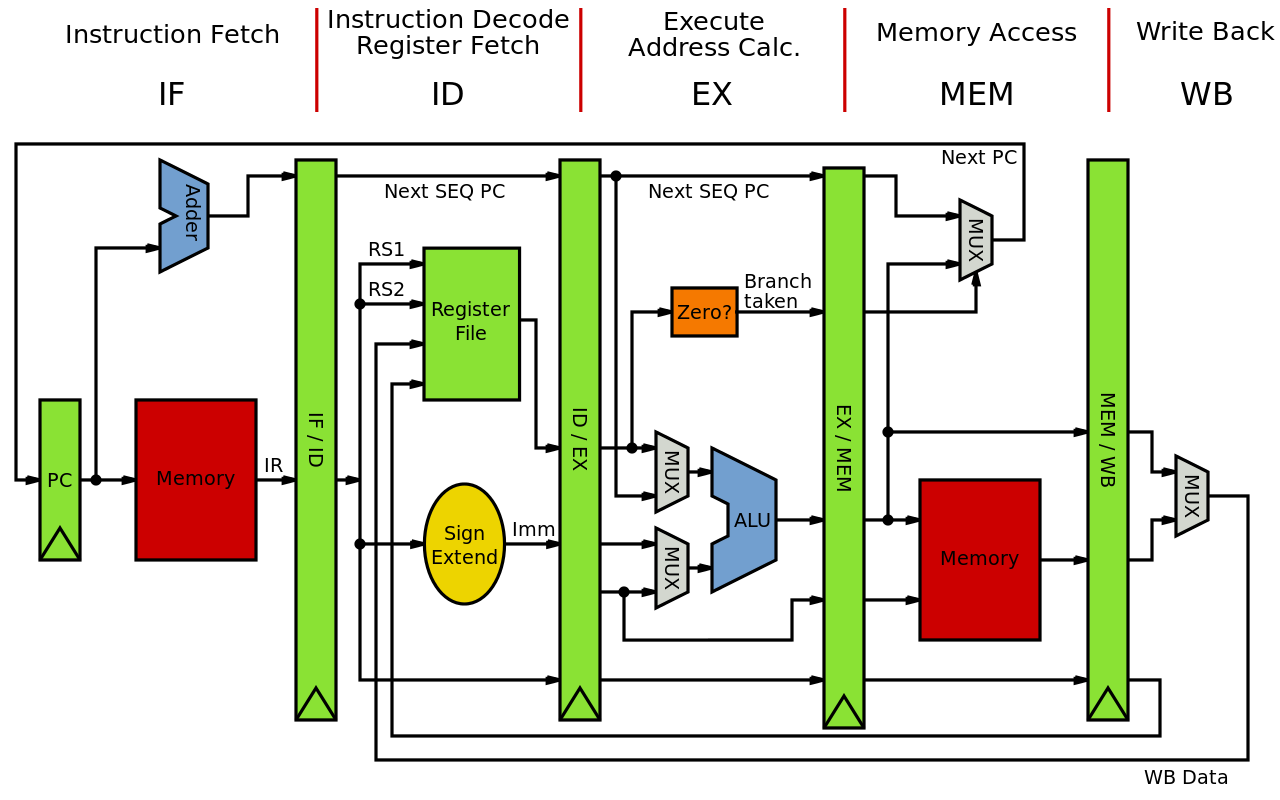
\includegraphics[width=\textwidth]{./mips-arch}

\tiny{\url{http://commons.wikimedia.org/wiki/File:MIPS_Architecture_(Pipelined).svg}}
\end{frame}

\begin{frame}{Проблемы}
\begin{itemize}
    \item Функциональная модель — не работает (слишком грубая)
    \item DES — применима, но неудобная абстракция
\end{itemize}

\input{../../simbook/metoda/drawings/des-long}

\end{frame}

\begin{frame}{Особенности}

\input{../../simbook/metoda/drawings/features}
\end{frame}

\begin{frame}{Проблемы}

Длительность одной операции у разных узлов
могут быть различными

 Как проверять готовность «медленных» узлов?
Результаты обработки данных должны появляться
не ранее, чем на такте, следующим за текущим

 Нельзя в произвольном порядке обновлять состояние
блоков

\end{frame}

\section{Порты}

\begin{frame}{Решение}
Абстрагируемся
Отделим:
●
 Функции узлов
●
 Время, затрачиваемое на их выполнение
●
 Внутреннее состояние узлов
ы
\end{frame}


\begin{frame}{Функциональный элемент}

Результат готов «мгновенно» при наличии
входных данных

\end{frame}

\begin{frame}{Порт}
Порт
Очередь фиксированной задержки
Ширина N бит, задержка 1 такт

\end{frame}

\begin{frame}{Правило соединения}

Функции не могут соединяться непосредственно друг с другом


\end{frame}

\begin{frame}{Модель с портами}

\end{frame}

\section{Детали}

\begin{frame}{Готовность данных}

\end{frame}

\begin{frame}{Стадии}


 симуляция функций

 симуляция передачи результатов

\end{frame}

\begin{frame}{Шаг 1, шаг 2}

\end{frame}


\begin{frame}{Могут ли функциональные элементы иметь память?}

\end{frame}

\begin{frame}{Связь функциональной и потактовой моделей}

\end{frame}

% \begin{frame}{Диаграмма моделируемой системы}
% 
% \end{frame}


\begin{frame}[allowframebreaks]{Литература}
\begin{thebibliography}{99}
    \bibitem{patterson-hennessy} Дэвид Паттерсон и Джон Хэннесси. Архитектура компьютера и проектирование компьютерных
систем. 4-е изд. Питер, 2012.

\bibitem{Asim} Joel Emer, Pritpal Ahuja, Eric Borch, Artur Klauser, Chi-Keung Luk, Srilatha Manne, Shubhendu S. Mukherjee,
Harish Patil, Steven Wallace, Nathan Binkert, Roger Espasa, Toni Juan. Asim: A Performance Model Framework // Computer 35 (2002), p. 68–76.

\bibitem{baida} Ю.В. Байда. Методы разработки и тестирования аппаратных потактовых моделей микропроцессоров на программируемых логических интегральных схемах. Дисс. к.т.н. — 2013
\end{thebibliography}
\end{frame}

\begin{frame}{На следующей лекции}
\centering

Параллельная симуляция, управляемая исполнением (MPonMP)

\end{frame}


\begin{frame}

{\huge{Спасибо за внимание!}\par}

\vfill

Слайды и материалы курса доступны по адресу \url{http://is.gd/ivuboc} % http://atakua.doesntexist.org/wordpress/simulation-course-russian/

\vfill

\tiny{\textit{Замечание}: все торговые марки и логотипы, использованные в данном материале, являются собственностью их владельцев. Представленная здесь точка зрения отражает личное мнение автора, не выступающего от лица какой-либо организации.}

\end{frame}

\end{document}
